\documentclass[a4paper,10pt]{article}
\usepackage[utf8]{inputenc}
\usepackage[brazil]{babel}
\usepackage{listings}
\usepackage{enumerate}
\usepackage{graphicx}


\begin{document}
\lstset{language=c,numbers=left,numberstyle=\tiny,breaklines=true,frame=single}

\begin{titlepage}

\begin{center}
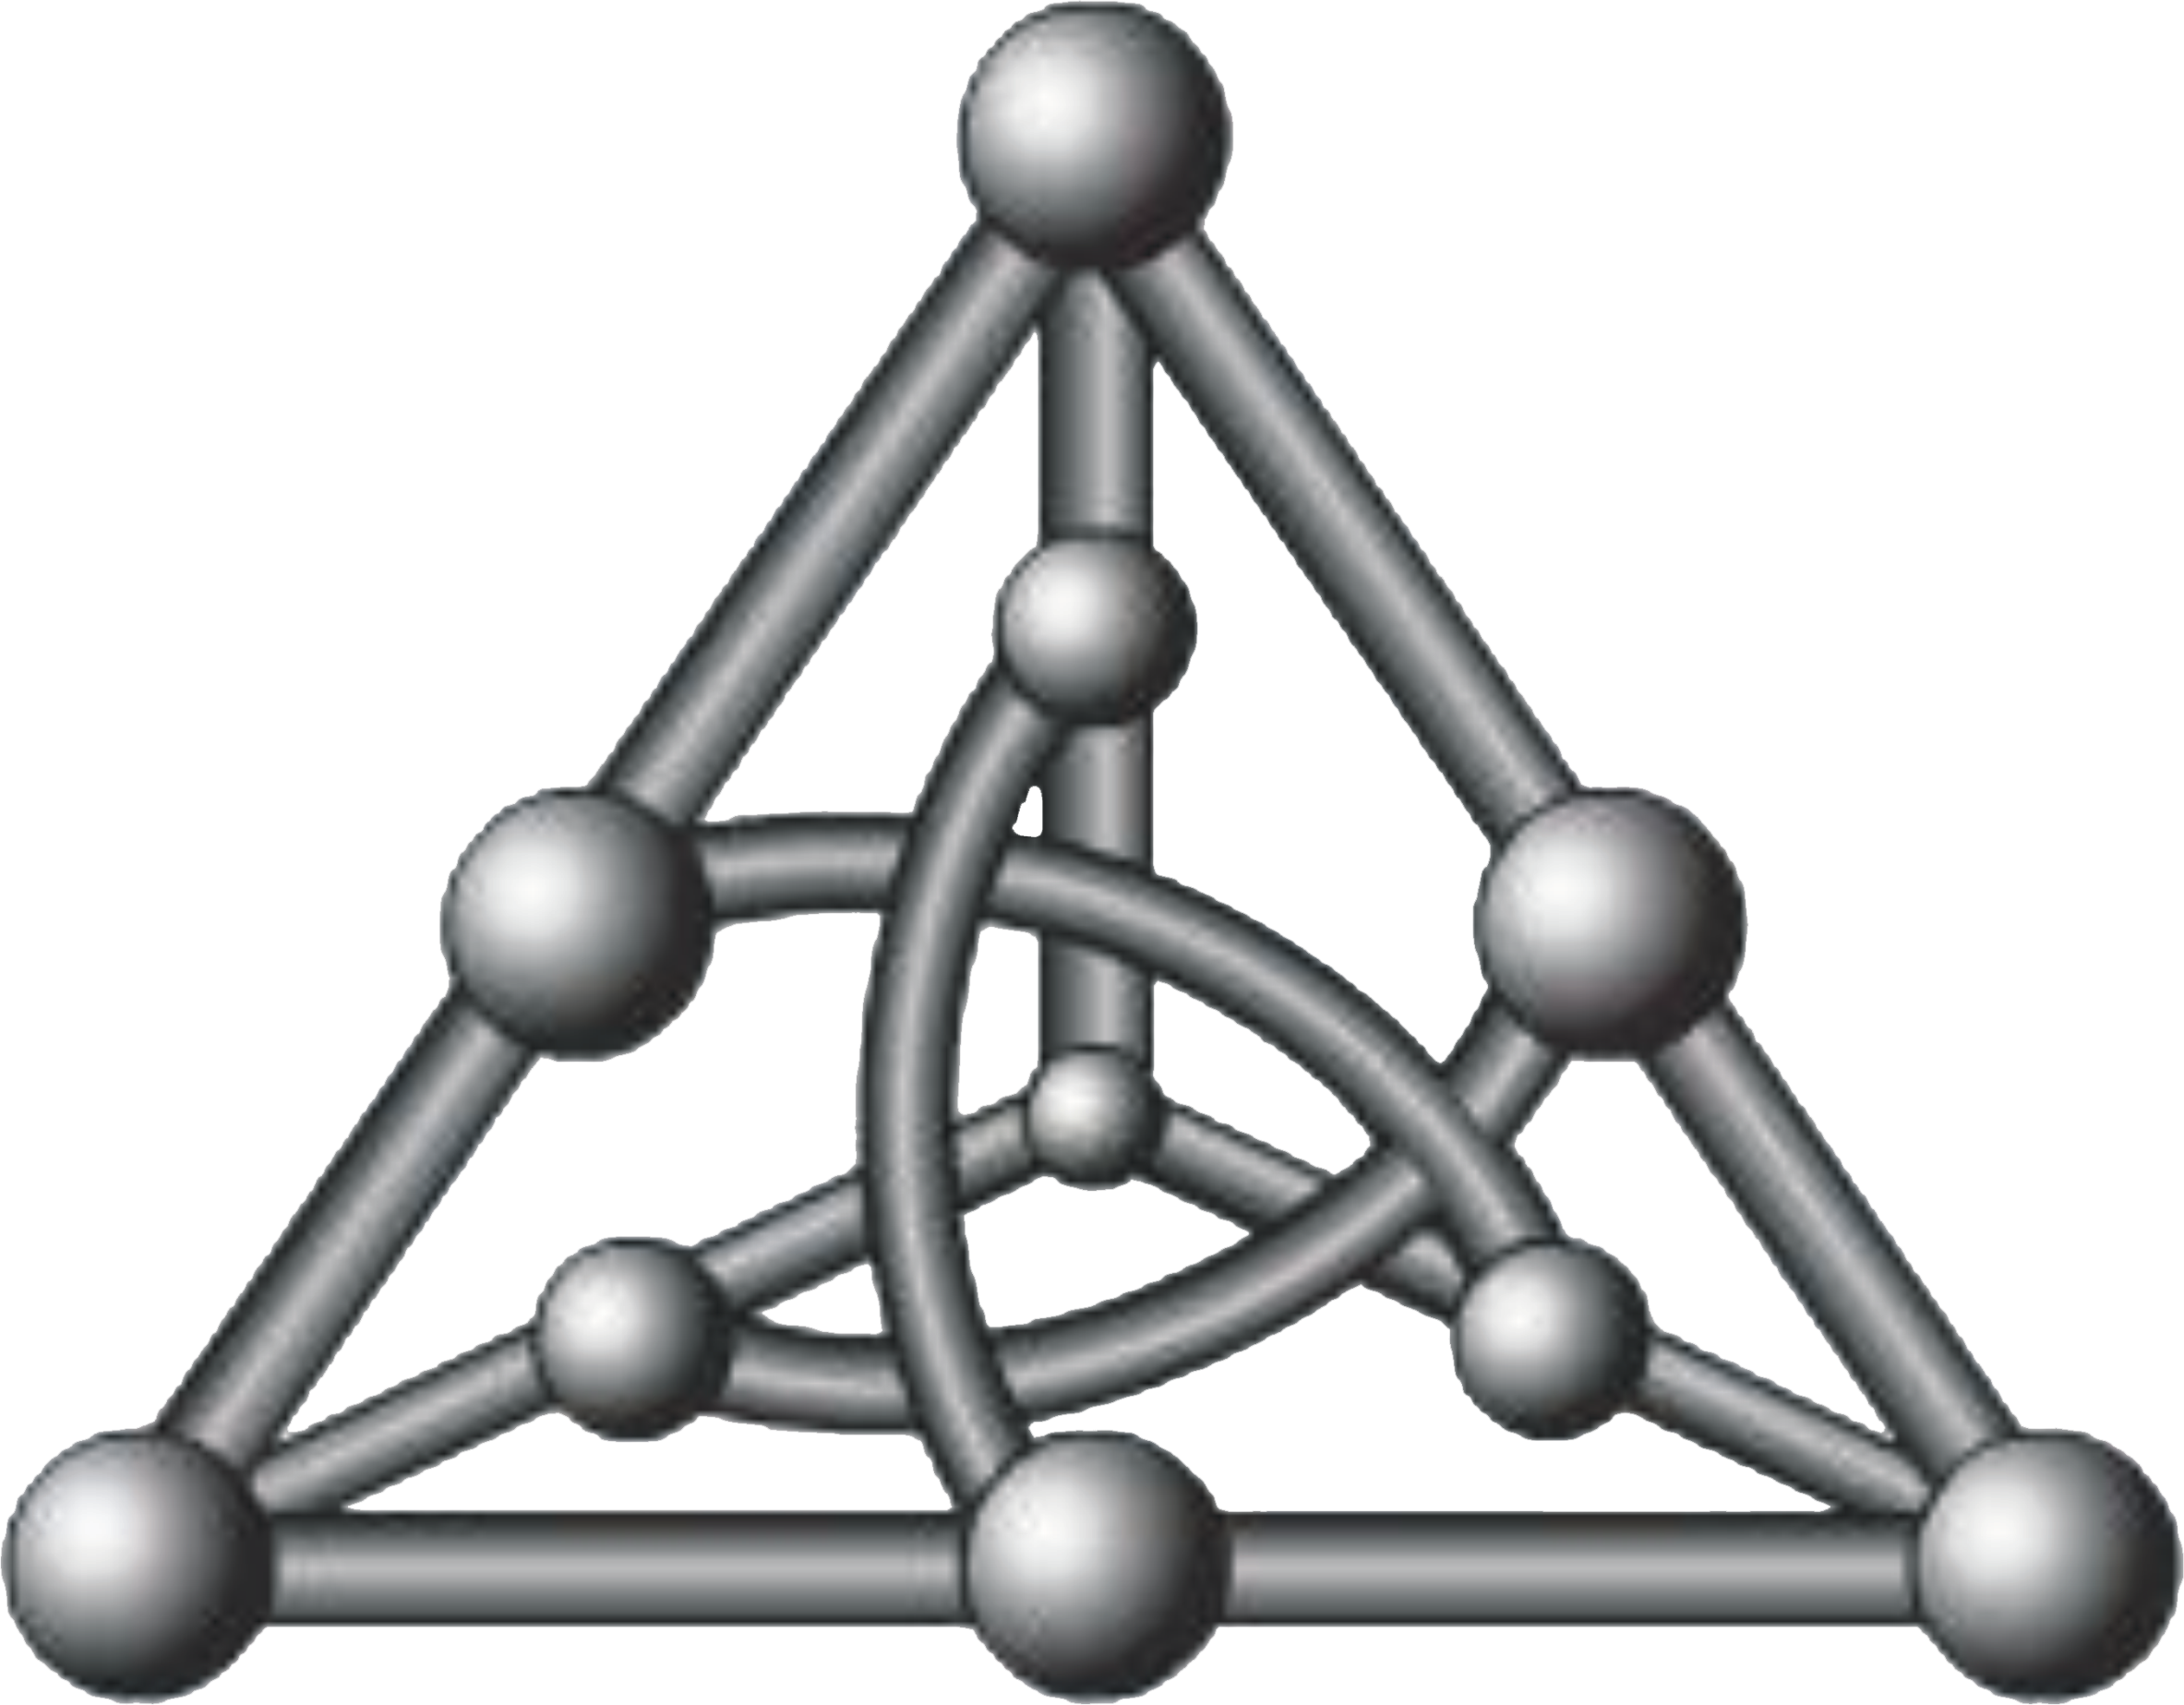
\includegraphics[width=2.5cm]{facom_t}\\[0.5cm]
\textsc{\LARGE Algoritimos de programação II}\\[0.5cm]
\textsc{Professor: Marco Aurélio Stefanes}\\[2.5cm]
{ \huge \bfseries Lista 01 \\[0.4cm] }
\end{center}
\vspace{10cm}


\begin{minipage}{1.6\textwidth}
\begin{center}
\emph{Aluno:} \\
Augusto Cesar de Aquino Ribas\\
Análise de Sistemas\\
\end{center}
\end{minipage}%

\end{titlepage}

\newpage
\section{Aula 01-03 : Exercícios. 1.5 a 1.9}

\begin{enumerate}

\item 
\begin{enumerate}[(a)]

\item Escreva uma função recursiva com a seguinte interface:\\

\begin{lstlisting}
int soma_digitos(int n)
\end{lstlisting}

que receba um número inteiro positivo $n$ e devolva a soma de seus dígitos.\\

\begin{lstlisting}
int soma_digitos(int n) {
  int soma;

  if((n/10)==0) {
    soma=n;
  } else {
    soma=n%10+soma_digitosR(n/10);
  }

  return soma;

}
\end{lstlisting}

\item Escreva um programa que receba um número inteiro $n$ 
e imprima a soma de seus dígitos. Use a função do item (a).\\

\begin{lstlisting}
#include <stdio.h>

int soma_digitos(int n) {
  int soma;
  if((n/10)==0) {
    soma=n;
  } else {
    soma=n%10+soma_digitosR(n/10);
  }
  return soma;
}

int main(void)
{
  int n;
  scanf("%d",&n);
  printf("Funcao recursiva: Soma dos digitos e %d\n",soma_digitos(n));
  return 0;
}
\end{lstlisting}
\end{enumerate} %letras
\pagebreak

\item  A \textbf{seqüência de Fibonacci} é uma seqüência de números inteiros positivos dada pela seguinte fórmula:
  \[ 
  \left\{ \begin{array}{rcl}
    F_1 & = & 1 \\
    F_2 & = & 1 \\
    F_i & = & F_{i-1} + F_{i-2},\ \textnormal{para}\ i\geq 3 
  \end{array}
  \right. 
  \]

\begin{enumerate}[(a)]
\item Escreva uma função recursiva com a seguinte interface:

\begin{lstlisting}
int Fib(int i)
\end{lstlisting}

que receba um número inteiro positivo $i$ e devolva o $i$-ésimo termo da seqüência de Fibonacci, isto é, $F_i$. 

\begin{lstlisting}
int fib(int i){

  if(i==1) {
    return 1;
  } else {
    if(i==2) {
      return 1;
    } else {
      return fib(i-1)+fib(i-2);
    }
  }
}
\end{lstlisting}
  
\item Escreva um programa que receba um número inteiro $i \geq 1$ e imprima o termo $F_i$ da seqüência de Fibonacci. 
Use a função do item (a).

\begin{lstlisting}
#include <stdio.h>

int fib(int i){
  if(i==1) {
    return 1;
  } else {
    if(i==2) {
      return 1;
    } else {
      return fib(i-1)+fib(i-2);
    }
  }
}

int main(void)
{
  int i;
  scanf("%d",&i);
  printf("Resultado = %d\n",fib(i));
  return 0;
}
\end{lstlisting}

\end{enumerate}
\pagebreak

\item O \textbf{piso} de um número inteiro positivo $x$ é o único inteiro $i$ 
tal que $i \leq x < i + 1$. O piso de $x$ é denotado por $\lfloor x \rfloor$.   

Segue uma amostra de valores da função $\lfloor \log_2 n \rfloor$:

  \begin{center}
    \begin{tabular}{*{13}{r}}
      $n$ & 15 & 16 & 31 & 32 & 63 & 64 & 127 & 128 & 255 & 256 & 511
      & 512 \\ \cline{2-13}  
      $\lfloor \log_2 n \rfloor$ & 3 & 4 & 4 & 5 & 5 & 6 & 6 & 7 & 7 &
      8 & 8 & 9  
    \end{tabular}
  \end{center}

\begin{enumerate}[(a)]
\item Escreva uma função recursiva com a seguinte interface:

\begin{lstlisting}
int piso_log2(int n)
\end{lstlisting}

que receba um número inteiro positivo $n$ e devolva $\lfloor
\log_2 n \rfloor$. 

\item Escreva um programa que receba um número inteiro $n \geq 1$ e imprima $\lfloor \log_2 n \rfloor$. 
Use a função do item (a). 
\end{enumerate}

\pagebreak

\item Considere o seguinte processo para gerar uma seqüência de números.
Comece com um inteiro $n$. Se $n$ é par, divida por $2$.
Se $n$ é ímpar, multiplique por $3$ e some $1$. 
Repita esse processo com o novo valor de $n$, terminando quando $n = 1$.
Por exemplo, a seqüência de números a seguir é gerada para $n = 22$:

  \[
  22 \hspace*{.5cm} 11 \hspace*{.5cm} 34 \hspace*{.5cm} 17 
  \hspace*{.5cm} 52 \hspace*{.5cm} 26 \hspace*{.5cm} 13 \hspace*{.5cm} 
  40 \hspace*{.5cm} 20 \hspace*{.5cm} 10 \hspace*{.5cm} 5
  \hspace*{.5cm} 16 \hspace*{.5cm} 8 \hspace*{.5cm} 4 \hspace*{.5cm} 2
  \hspace*{.5cm} 1   
  \]

É conjecturado que esse processo termina com $n = 1$ para todo inteiro $n > 0$.
Para uma entrada $n$, o \textbf{comprimento do ciclo de $n$} é o número de elementos gerados na seqüência.
No exemplo acima, o comprimento do ciclo de $22$ é $16$. 

\begin{enumerate}[(a)]
  \item Escreva uma função não-recursiva com a seguinte interface:

\begin{lstlisting}
int ciclo(int n)
\end{lstlisting}

que receba um número inteiro positivo $n$, mostre a seqüência gerada pelo processo descrito acima 
na saída e devolva o comprimento do ciclo de $n$. 

\begin{lstlisting}
int ciclo(int n){
  int ciclo=1;
  while(n!=1) {
    if(n%2==0) {
      printf("%d ",n/2);
      n=n/2;
    } else {
      printf("%d ",n*3+1);
      n=n*3+1;
    }
    ciclo++;
  }
  return ciclo;
}
\end{lstlisting}

\pagebreak

\item Escreva uma versão recursiva da função do item (a) com a seguinte interface: 

\begin{lstlisting}
int cicloR(int n)
\end{lstlisting}

que receba um número inteiro positivo $n$, mostre a seqüência gerada pelo processo descrito 
acima na saída e devolva o comprimento do ciclo de $n$.

\begin{lstlisting}
int cicloR(int n){
  if(n%2==0) {
    printf("%d ",n/2);
    n=n/2;
  } else {
    printf("%d ",n*3+1);
    n= n*3+1;
  }
  if(n==1) {
    return 2;
  } else {
    return 1+cicloR(n);
  }
}
\end{lstlisting}
\pagebreak

\item Escreva um programa que receba um número inteiro $n \geq 1$ e determine a seqüência gerada 
por esse processo e também o comprimento do ciclo de $n$. Use as funções em (a) e (b) para testar. 
\end{enumerate}

\begin{lstlisting}
#include <stdio.h>

int ciclo(int n){
  int ciclo=1;
  while(n!=1) {
    if(n%2==0) {
      printf("%d ",n/2);
      n=n/2;
    } else {
      printf("%d ",n*3+1);
      n=n*3+1;
    }
    ciclo++;
  }
  return ciclo;
}
int cicloR(int n){
  if(n%2==0) {
    printf("%d ",n/2);
    n=n/2;
  } else {
    printf("%d ",n*3+1);
    n= n*3+1;
  }
  if(n==1) {
    return 2;
  } else {
    return 1+cicloR(n);
  }
}

int main(void)
{
  int x, saida;
  scanf("%d",&x);
  saida=ciclo(x);
  printf("\niterativo %d\n",saida);
  saida=cicloR(x);
  printf("\nrecursivo %d\n",saida);
  return 0;
}
\end{lstlisting}
\pagebreak


\item Podemos calcular a potência $x^n$ de uma maneira mais eficiente.
Observe primeiro que se $n$ é uma potência de 2 então $x^n$ pode ser computada usando seqüências de quadrados.
Por exemplo, $x^4$ é o quadrado de $x^2$ e assim $x^4$ pode ser computado usando somente duas multiplicações 
ao invés de três. Esta técnica pode ser usada mesmo quando $n$ não é uma potência de 2, usando a seguinte fórmula:


\[    x^n = \left \{ \begin{array}{ll}
        1\:, & \textnormal{se $n = 0$,} \\
        (x^{n/2})^2\:, & \textnormal{se $n$ é par,} \\
        x \cdot x^{n-1}\:, & \textnormal{se $n$ é ímpar.}
      \end{array} \right. \]

  
  
  
  
  \begin{enumerate}[(a)]
  \item Escreva uma função com interface

\begin{lstlisting}
int potencia(int x, int n)
\end{lstlisting}

que receba dois números inteiros $x$ e $n$ e calcule e devolva $x^n$ usando a fórmula acima.

\begin{lstlisting}
int potencia(int x, int n) {
  int num;
  if(n==0) {
    printf("N e %d \n",n);
    /*Se n e zero*/
    return 1;
  } else {
    if( (n%2) == 0 ) {
      printf("N e %d \n",n);
    /*Se n e par*/
      num=potencia(x,n/2);
      return num*num;
    } else {
      printf("N e %d \n",n);
    /*Se n e impar*/
      return x * potencia(x,n-1);
    }
  }
}
\end{lstlisting}

\pagebreak

\item Escreva um programa que receba dois números inteiros $a$ e $b$ e imprima o valor de $a^b$.
  \end{enumerate}
  
\begin{lstlisting}
#include <stdio.h>

int potencia(int x, int n) {
  int num;
  if(n==0) {
    printf("N e %d \n",n);
    /*Se n e zero*/
    return 1;
  } else {
    if( (n%2) == 0 ) {
      printf("N e %d \n",n);
    /*Se n e par*/
      num=potencia(x,n/2);
      return num*num;
    } else {
      printf("N e %d \n",n);
    /*Se n e impar*/
      return x * potencia(x,n-1);
    }
  }
}

int main(void) {
  int num, pot;
  scanf("%d %d",&num, &pot);
  printf("Resposta: %d\n",potencia(num,pot));
  return 0;
}
\end{lstlisting}

\end{enumerate} %Números
\pagebreak



\newpage
\section{Aula 05: Exercícios 2.6 a 2.10}

\begin{enumerate}
 
 
\item É verdade que $2^{n+1} = O(2^n)$? E é verdade que $2^{2 \cdot n} = O(2^n)$?

\item Suponha que você tenha algoritmos com os cinco tempos de execução listados abaixo.
Quão mais lento cada um dos algoritmos fica quando você (i) duplica o tamanho da
entrada, ou (ii) incrementa em uma unidade o tamanho da entrada?

  \begin{enumerate}[(a)]
\item $n^2$
\item $n^3$
\item $100 \cdot n^2$
\item $n \cdot \log_2(n)$
\item $2^n$
  \end{enumerate}

\item Suponha que você tenha algoritmos com os seis tempos de execução listados abaixo. Su-
ponha que você tenha um computador capaz de executar 1010 operações por segundo
e você precisa computar um resultado em no máximo uma hora de computação. Para
cada um dos algoritmos, qual é o maior tamanho da entrada n para o qual você poderia
receber um resultado em uma hora?

  \begin{enumerate}[(a)]
\item $n^2$
\item $n^3$
\item $100\cdot n^2$
\item $n\cdot \log_2(n)$
\item $2^n$
\item $2^{2^n}$

  \end{enumerate}

\item Rearranje a seguinte lista de funções em ordem crescente de taxa de crescimento. Isto é,
se a função $g(n)$ sucede imediatamente a função $f(n)$ na sua lista, então é verdade que $f(n) = O(g(n))$.


\begin{center}
 
$f1(n) = n^{2.5}$ \linebreak
$f2(n) = \sqrt{2\cdot n}$ \linebreak
$f3(n) = n + 10$ \linebreak
$f4(n) = 10^n$ \linebreak
$f5(n) = 100^n$ \linebreak
$f6(n) = n^2 \cdot \log_2(n)$ \linebreak

\end{center}

\item Considere o problema de computar o valor de um polinômio em um ponto. 
Dados n coeficientes $a_0 , a_1 , . . . , a_{n-1}$ e um número real $x$, queremos computar $\Sigma_{i=0}^{n-1} a_i \cdot x^i$.
  
  \begin{enumerate}[(a)]
\item Escreva um programa simples com tempo de execução de pior caso $O(n^2)$ para solucionar este problema.
\item Escreva um programa com tempo de execução de pior caso $O(n)$ para solucionar este problema 
usando o método chamado de regra de Horner para reescrever o polinômio:
  \end{enumerate}



\item Seja $A[0...n-1]$ um vetor de $n$ números inteiros distintos dois a dois. Se $i<j$ e $A[i]>A[j]$
então o par $(i,j)$ é chamado uma inversão de A.

  \begin{enumerate}[(a)]
\item Liste as cinco inversões do vetor $A = 2, 3, 8, 6, 1$ .
\item Qual vetor com elementos no conjunto ${1, 2, . . . , n}$ tem a maior quantidade de in-
versões? Quantas são?
\item Escreva um programa que determine o número de inversões em qualquer permuta-
ção de n elementos em tempo de execução de pior caso $O(n \cdot \log_2(n))$.
  \end{enumerate}
  
\end{enumerate} %Números

\end{document}
